\section{Visualisations - Chaleur}

Les figures ci-dessous montrent la distribution de la chaleur dans
l'enceinte du four vide, et dans l'enceinte du four avec l'aliment
dedans.

La source du champ magnétique se trouve à gauche dans toutes les
figures, et on impose ici $g = 0$ sur toutes les autres parois
du four.

Voir les sections~\ref{experiences_numeriques:constantes}
et~\ref{experiences_numeriques:dimensions_four} pour consulter
les valeurs des paramètres physiques et les dimensions du four.

\begin{figure}[H]
    \centering
    \begin{subfigure}{.5\textwidth}
        \centering
        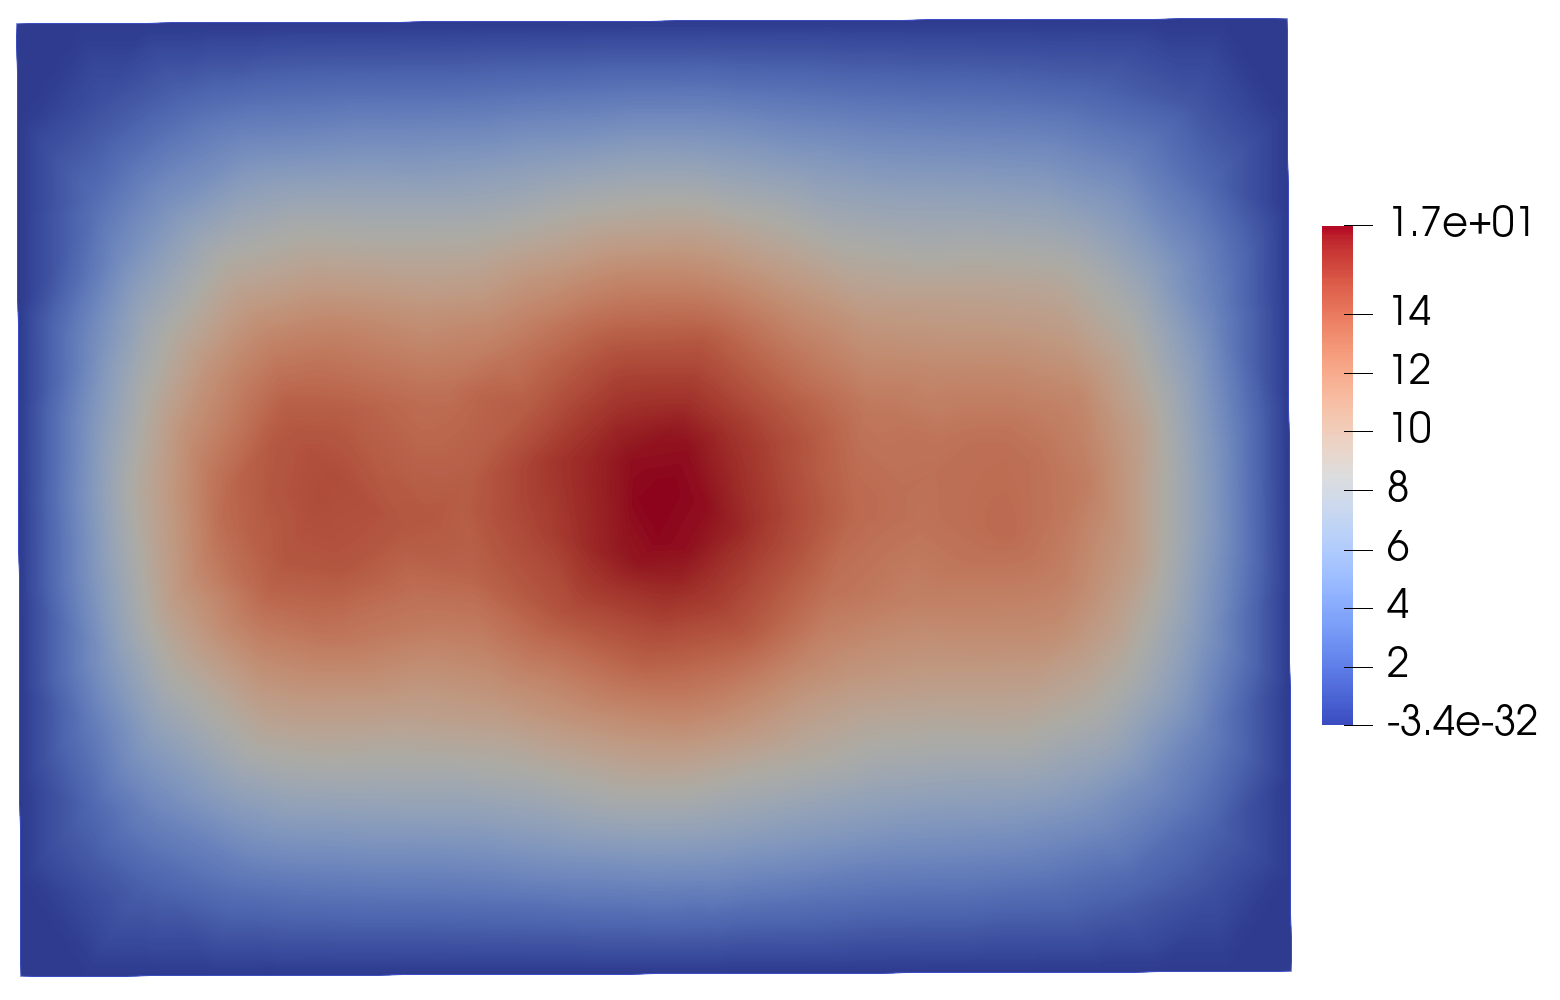
\includegraphics[scale=0.15]{figures/chaleur/chaleur_vide1.png}
    \end{subfigure}%
    \begin{subfigure}{.5\textwidth}
        \centering
        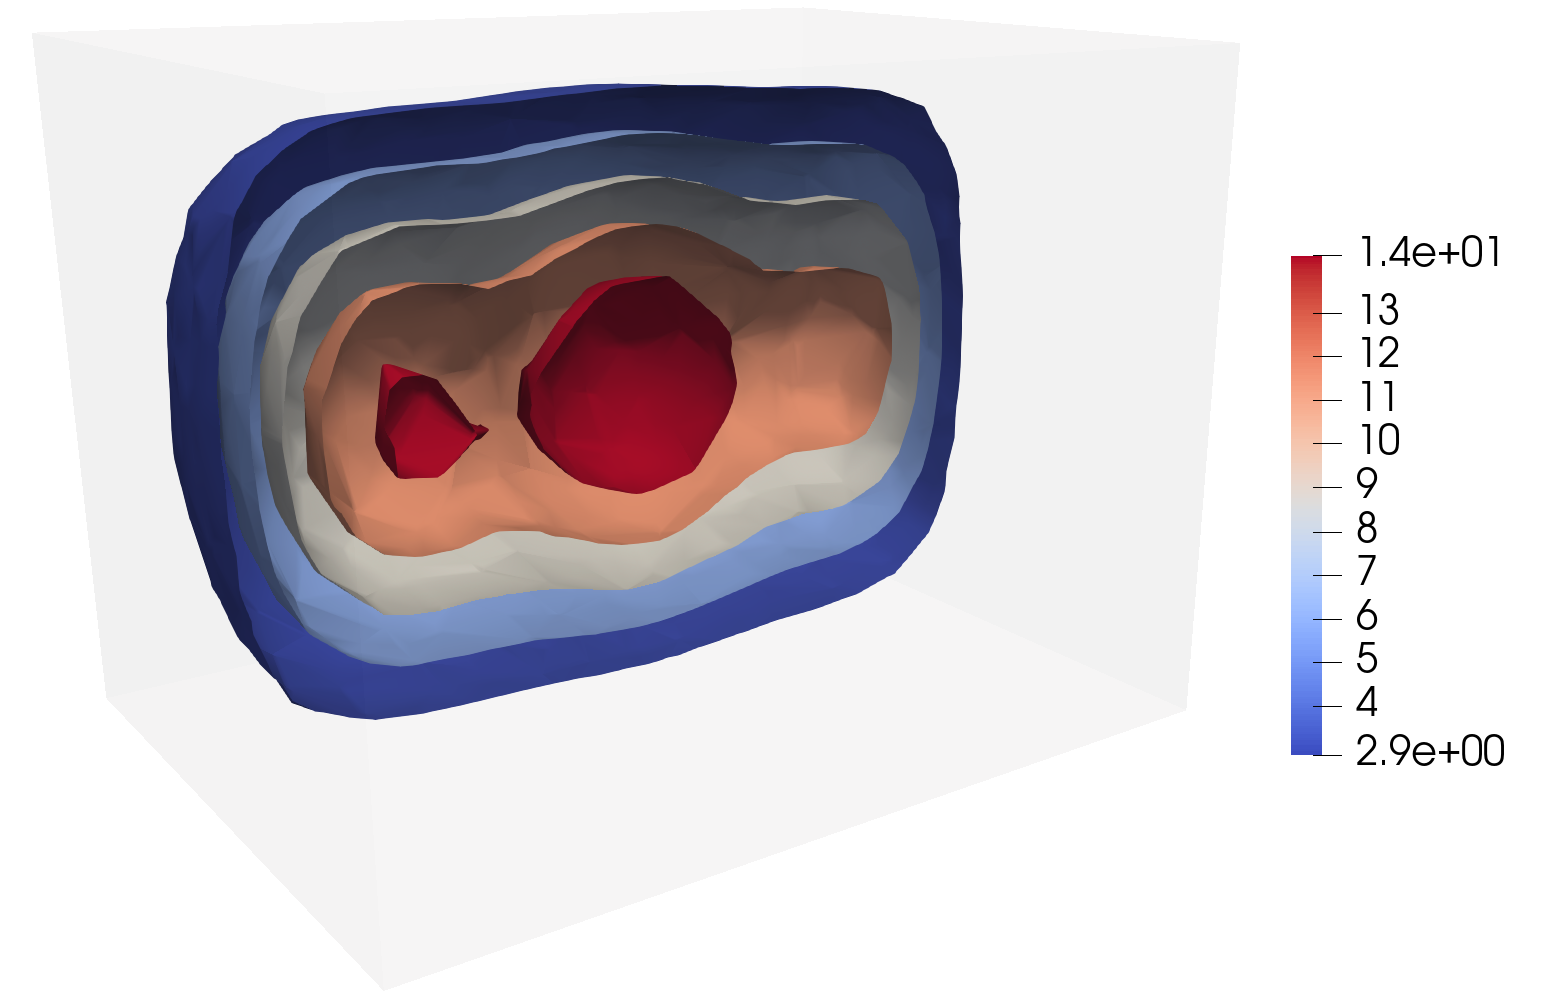
\includegraphics[scale=0.15]{figures/chaleur/chaleur_vide2.png}
    \end{subfigure}
    \caption{La distribution de la chaleur dans l'enceinte du four vide.
    À gauche : une tranche prise au milieu de l'enceinte sur l'axe $x$.
    À droite : un clip des tracés de contours.}
\end{figure}

\begin{figure}[H]
    \centering
    \begin{subfigure}{.5\textwidth}
        \centering
        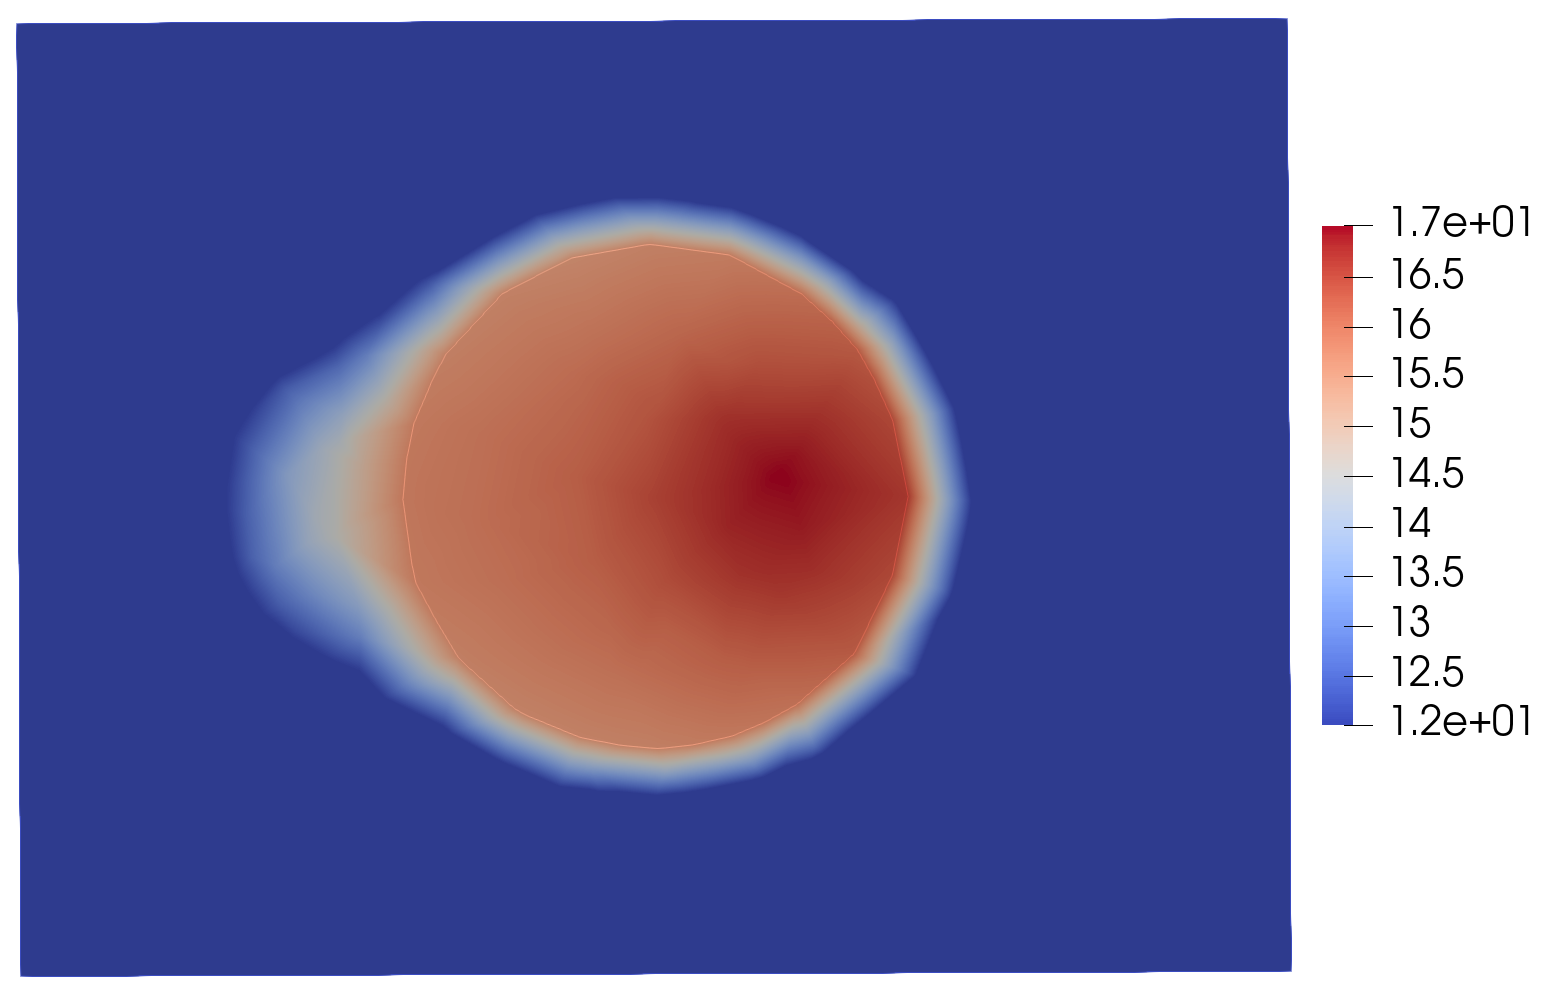
\includegraphics[scale=0.15]{figures/chaleur/chaleur1.png}
    \end{subfigure}%
    \begin{subfigure}{.5\textwidth}
        \centering
        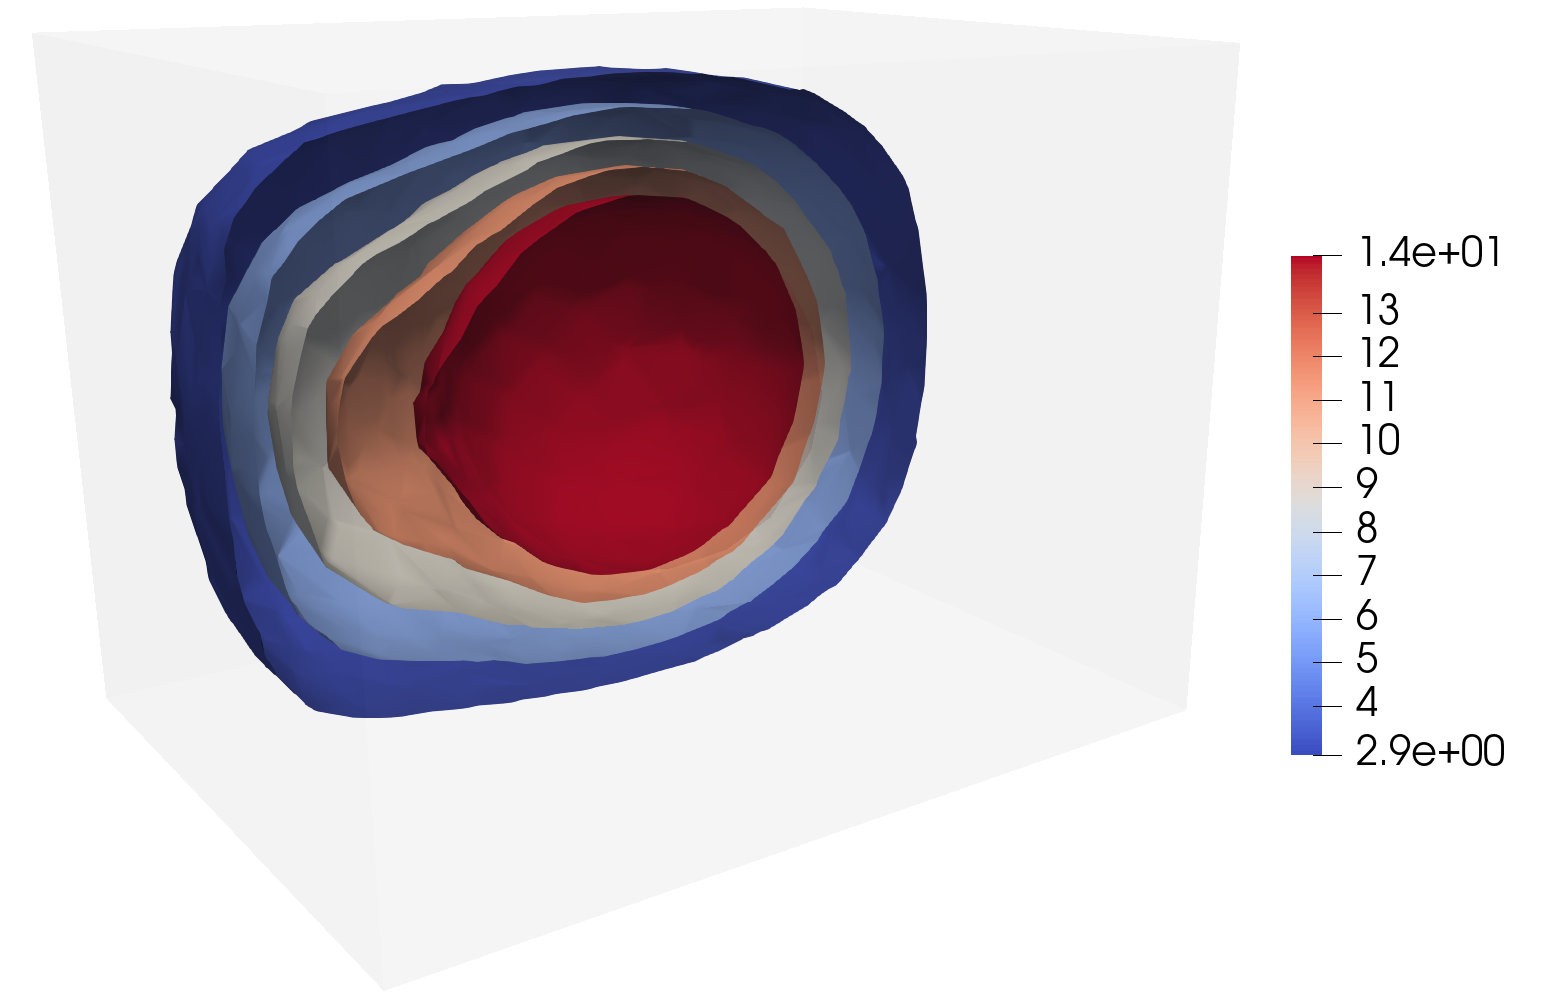
\includegraphics[scale=0.15]{figures/chaleur/chaleur2.png}
    \end{subfigure}
    \caption{La distribution de la chaleur dans l'enceinte du four
    avec l'aliment dedans.
    À gauche : une tranche prise au milieu de l'enceinte sur l'axe $x$.
    À droite : un clip des tracés de contours.}
\end{figure}
